\chapter{Brudgrænsetilstand}
INDLEDNING

\section{Reaktioner}
Når der beregnes reaktionskræfter for de tre understøtninger, er der behov for at opdele konstruktionen. Systemet opdeles i det midterste charnierled i henholdvis en venstre- og højre del, som ses på Figur \ref{fig:opdelingv} og \ref{fig:opdelingh}. I skæringen mellem de to dele, vil der være snitkræfter men ikke momentkræfter, da momentet i charnierledet er nul. Dermed optræder der kun normalkraften, N, og forskydningskraften, V.

\begin{figure}[htbp]\centering
	\begin{minipage}[b]{0.48\textwidth}\centering
		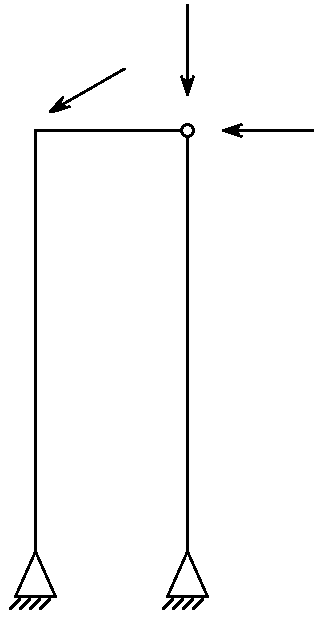
\includegraphics[width=0.50\textwidth]{billeder/venstre.png} %Venstre billede
	\end{minipage}\hfill
	\begin{minipage}[b]{0.48\textwidth}\centering
		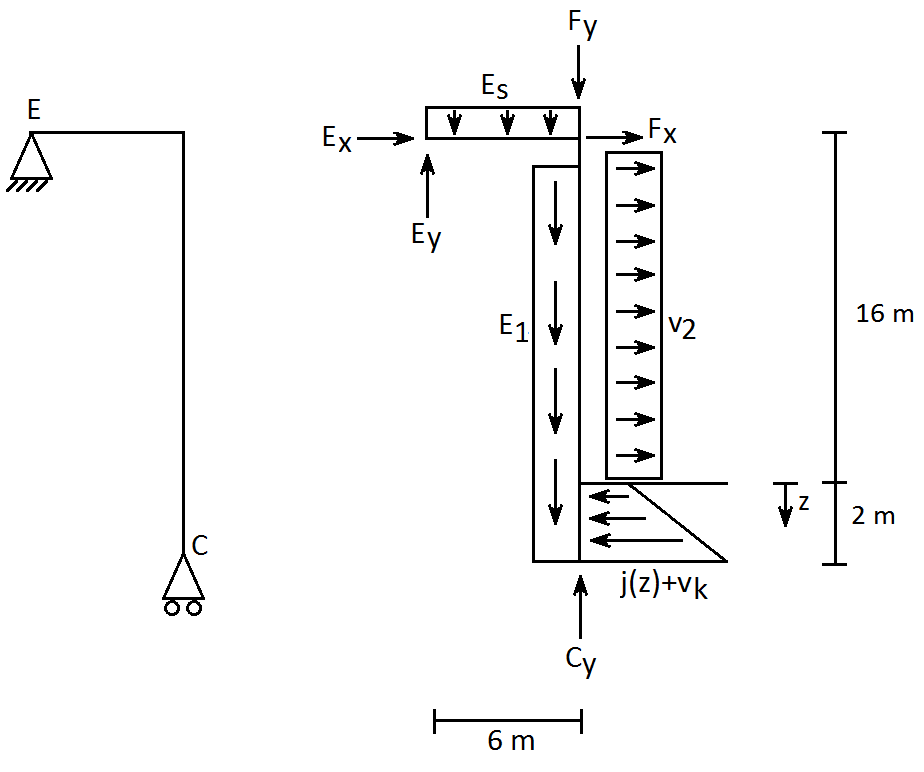
\includegraphics[width=0.35\textwidth]{billeder/hojre.png} %Højre billede
	\end{minipage}\\ %Captions and labels
	\begin{minipage}[t]{0.48\textwidth}
		\caption{Venstre side af systemet} %Venstre caption og label
		\label{fig:opdelingv}
	\end{minipage}\hfill
	\begin{minipage}[t]{0.48\textwidth}
		\caption{Højre side af systemet} %Højre caption og label
		\label{fig:opdelingh}
	\end{minipage}
\end{figure}

Reaktionerne, der vil virke i charnieret, sættes som belastninger på venstre del af systemet. 
\newline
\newline
Reaktionerne på højre del af systemet beregnes først.
\newline
\newline
Lasterne, der påvirker højre side af det statiske system, ses på Figur XX, hvor værdierne kan ses i Tabel \ref{tab:laster}.
% Indsæt figur med hvordan lasterne er på venstre- og højre del af systemet.

\begin{table}
	\begin{center}
		\begin{tabular}{|c|c|c|}
			\hline
Betegnelse     & Værdi & Enhed \\ \hline
$P_1$           &       &       \\ \hline
$P_2$           &       &       \\ \hline
$q_1$           & 31,54 & $\frac{kN}{m}$ \\ \hline
$q_2$           & 9,47  & $\frac{kN}{m}$ \\ \hline
$q_3$           & 61,34 & $\frac{kN}{m}$ \\ \hline
$Vind_1$        & 6,08  & $\frac{kN}{m}$ \\ \hline
$Vind_2$       	& -1,20 & $\frac{kN}{m}$ \\ \hline
$Jord+vind_ind$ & $63,\!77x + 1,\!66$ & $\frac{kN}{m}$ \\ \hline
		\end{tabular}
		\caption{Laster på det statiske system}
		\label{tab:laster}
	\end{center}
\end{table}

Først bestemmes $Cha_v$ gennem vandret ligevægt: 
\begin{center}
	$\rightarrow+:0=F_x+Cha_v-J(2m)-V_k\cdot2m-V_2\cdot16m$
	$Cha_v\leftrightarrow -27349,37742$
\end{center}

Nu bestemmes $C_y$ gennem moment ligevægt: 
\begin{center}
	$\AR{}:0=-F_y\cdot6m-E_1\cdot18m\cdot6m+C_y\cdot6m-J(2m)\cdot17,\!33m-V_k\cdot2m\cdot17m-E_s\cdot6m\cdot3m-V_2\cdot16m\cdot8m$
	$C_y\leftrightarrow 8,\!064541700\cdot10^5N$ 
\end{center}

Nu kan $Cha_l$ bestemmes gennem lodret ligevægt: 
\begin{center}
	$\uparrow+:0=F_y-E_1\cdot18m-E_s\cdot6m+C_y+Cha_l$
	$Cha_l \leftrightarrow -2,\!976261656*10^5N$
\end{center}

Der beregnes nu på systemet til venstre da reaktionerne i charnieret er fundet, disse bliver sat som belastninger som ses på billede (blabla 4)

%indsæt Figur 

Der startes her med at beregne moment omkring A da der i denne ligninge kun vil være en ubekendt som er $B_{lodret}$  
\begin{center}
	$A\hookrightarrow+:0=B_y*6m+Charnier_Lodret*6m+-18m*Charnier_vandret-E*18m*6m-d*18m*6m-d*18m*6-d-18m-E*6m*\frac{6}{2}+P_2*Cos(26,\!6)*18m-Vind_2*18m*(\frac{16}{2}m+2m)-\frac{J*2m}{2}*(\frac{2m}{2})$
	$B_y=\frac{1}{6m}*(-Charner_lodret*6m+18m*Charnier_vandret+E*18m*6m+d*18m*6m+d*18m*6m+d*18m+E*6m*\frac{6}{2}m-P_2*Cos(26,\!6)*18m+Vind_2*18m*(8m+2m+\frac{J*2m}{2}*\frac{2m}{2})$
\end{center}

Der regnes derefter på den lodrette ligevægt for at finde $A_{lodret}$
\begin{center}
	$\uparrow+:0=A_y+B_y+Charnier_y-E*18m-d*18m-d*18m-d*18m-E*6m-P_2*Sin(26,\!6)$
	$A_y=-B_y-Charnier_y+E*18m+d*18m+d*18m+d*18m+E*6m+P_2*Sin(26,\!6)$
\end{center}

For at gøre det muligt at isolere en af de vandrette reaktioner laves der et snint i charnieret og derefter bliver der taget moment omkring charnieret. Dette gøres for at finde $B_{vandret}$.
\begin{center}
	$\hookrightarrow+:0=18m*B_x+d*18m-d*18m$
	$B_x=\frac{d*18m-d*18m}{18m}=0$
\end{center}

Til sidst bruges den vandrette ligevægt til at finde $A_{vandret}$.
\begin{center}
	$\rightarrow+:0=A_x+Charnier_x+B_x+\frac{J*2m}{2}+Vind_2*16m-P_2*Cos(26,\!6)$
	$A_x=P_2*Cos(26,\!6)-Charnier_x-B_x-Vind_2*16m-\frac{J*2m}{2}$
\end{center} 
 
\section{Snitkræfter}
Både snitkræfter og snitkræftskurver.

\section{Spænding}
Spændingsfordeling af normalspænding og forskydningsspænding.

\section{...}
Brudgrænsetilstand, nedbøjning mm?...